\chapter{Metodologia}

Como todos os projetos de software bem estruturados e desenhados, serão utilizadas práticas e metodologias já existentes e comprovadas no mundo real. Neste capítulo irão ser demonstrados alguns dos elementos utilizados.

\section{Iterative and Incremental development}

Esta prática consiste numa combinação de práticas incrementais e iterativas, onde essencialmente um produto de software é separado em componentes, sendo que cada um destes componentes é iterativamente implementado. Essencialmente, esta metodologia de desenvolvimento irá ter os seguintes passos, para a elaboração de cada componente:
\begin{itemize}
    \item Requisitos - definição dos requisitos do sistema
    \item Design/Arquitetura - desenho da arquitetura do sistema
    \item Implementação - implementação dos elementos definidos na arquitetura
    \item Testes - testes unitários e de integração
    \item Avaliação - avaliação do sistema dum ponto de vista funcional e técnico
\end{itemize}

Durante a idealização da arquitetura, o sistema irá ser dividido em pequenos componentes ou sistemas que resultam no projeto final, sendo que cada um sistema irá ser implementado um de cada vez, seguindo esta metodologia. Na essência, esta metodologia é uma combinação da metodologia \textit{Waterfall} e incremental, desenvolvendo pequenas partes do sistema de cada vez.

\section{Model Driven Development}

Ideal para sistemas de grande complexidade, durante o desenvolvimento dos componentes de software deste projeto irão ser utilizados diagramas para descrever o comportamento do sistema num alto nível. Utilizando modelos de domínio e diagramas de classe, entre outros, será possível descrever a um alto nível de abstração, a estrutura e o comportamento do sistema de software antes da sua implementação.

Esta metodologia tem grandes vantagens, sendo uma delas a facilitação do trabalho em equipa e a colaboração com outros, uma vez que é mais fácil explicar conceitos através de um diagrama em vez de um excerto de código. Além disso, dado que os diagramas não estão necessariamente ligados a uma dada tecnologia ou linguagem de programação, teremos uma grande vantagem na altura de migrar o sistema para outra tecnologia, caso seja necessário. Além disso, existem aplicações no mercado, capazes de transformar modelos em código, reduzindo o tempo de implementação necessário.

Neste preciso caso, será utilizado UML para desenhar os diagramas, uma linguagem de modelação bastante utilizada na indústria, possuindo várias ferramentas capazes de transformar diagramas em código.

\section{Static Code Analysis}

Sistemas de software de  grande dimensão devem seguir os mesmos standards sintáticos e arquiteturais em toda o código. Para efetuar esta verificação, foram utilizadas ferramentas de análise de código, que permitem detetar \textit{code smells} e más práticas arquiteturais para prevenir \textit{bugs} e falhas de segurança. Também ajudam a manter o estilo do código uniforme, para melhorar a sua legibilidade e compreensibilidade.

\section{Continuous Integration}

Todos os componentes do sistema irão ser mantidos num sistema de controlo de versões, nomeadamente o \textit{git}, utilizando o serviço de \textit{hosting} do \textit{GitHub}, para manter todos os repositórios na \textit{cloud}. Utilizando o \textit{GitHub}, é possível efetuar várias integrações com outras ferramentas de \textit{testing} e \textit{deployment} que nos permitem seguir esta metodologia de \textit{continuous integration}.

\textit{Continuous integration} é o nome que se dá à prática de continuamente testar e integrar o código do software nos sistemas onde eles irão operar. O \textit{workflow} utilizado irá fazer uso do \textit{GitHub}, um sistema de \textit{hosting} de \textit{git}, o sistema de controlo de versões a ser utilizado, e, finalmente, do \textit{Travis}, uma plataforma de execução de testes automáticos.

Utilizando estes recursos é possível testar a última versão do código assim que ele é \textit{pushed} para o repositório remoto. Basicamente, assim que um novo \textit{commit} é \textit{pushed} para o \textit{GitHub}, o \textit{Travis} corre os testes dessa nova versão do software, reportando o resultado para o \textit{GitHub}. Além dos testes, também são executadas nesta fase as ferramentas de análise de código, retornando uma \textit{build} errónea caso elas detetem problemas.

\begin{figure}[H]
  \centering
        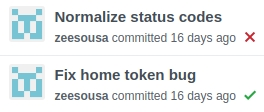
\includegraphics[scale=1]{img/github.jpg}
  \caption{Integração Travis \& GitHub}
\end{figure}

Neste exemplo, o \textit{commit} ''Fix home token bug'' passou os testes definidos enquanto que o último \textit{commit} ''Normalize status codes'' falhou os testes.

Os componentes do sistema que necessitarem de um sistema de \textit{hosting} irão recorrer ao \textit{Heroku}, uma \textit{platform as a service}, que permite correr qualquer tipo de serviço web sem custos. A única limitação consiste no adormecimento dos serviços, ou seja, todos os serviços grátis ''adormecem'' ao fim de 30 minutos sem receberem qualquer tráfego.

O \textit{Heroku} é semelhante ao \textit{Travis} na medida em que sempre que deteta um novo \textit{commit} no \textit{GitHub} tenta efetuar o \textit{deploy} dessa nova versão. Neste caso, como também temos o \textit{Travis} no nosso \textit{workflow}, o \textit{Heroku} aguarda que os testes passem antes de dar \textit{deploy} ao código. Assim, asseguramos que temos sempre uma versão estável do sistema ativa. 

É possível definir \textit{pipelines} avançadas no \textit{Heroku}, podendo ter sistemas de \textit{staging} e sistemas de \textit{production} ao mesmo tempo. Por exemplo, um sistema de \textit{staging} pode ter passado nos testes mas ainda está na fase de avaliação, enquanto que um sistema de \textit{production} já está pronto para utilização final. Além disso, também é possível ter uma aplicação por cada \textit{feature branch} presente no \textit{GitHub}, criando uma aplicação para cada \textit{pull request} ativo. Neste caso, temos apenas uma aplicação de \textit{staging} e uma para cada \textit{pull request} ativo.


